\documentclass[11pt,a4paper]{article}
\usepackage[utf8]{inputenc}
\usepackage{amsmath, amssymb}
\usepackage{graphicx}
\usepackage{booktabs}
\usepackage{geometry}
\geometry{margin=1in}

\title{Smart Evacuation of Multi-Floor Buildings using Crowd Dynamics and Optimization}
\author{Ghiffary Rifqialdi, Mohammed Kaif Khan, Muhammad Awais, Sadeeq Alam\\[1ex] \normalsize Department of Mathematics, University of Hamburg, Hamburg, Germany\\ \normalsize grifqialdi@gmail.com}
\date{16 July 2025}

\begin{document}
\maketitle

\begin{abstract}
Ensuring the safe and rapid evacuation of occupants from multi-floor buildings during emergencies is a critical challenge in building design and emergency management. In this paper, we present a hybrid approach combining a microscopic crowd dynamics model with a mesoscopic network flow model to simulate and optimize emergency evacuations in a two-story building under various hazard scenarios (normal conditions, fire, and earthquake). The microscopic model uses a Social Force paradigm to capture individual agent motions and local interactions, while the mesoscopic model represents pedestrian flow through a network of corridors, stairwells, and exits. We incorporate dynamic hazards such as spreading fire, smoke, and earthquake-induced debris into the simulation, affecting agent behavior and route availability in real-time. Furthermore, we formulate a layout optimization problem that adjusts building design variables (exit placements, stair locations, and door widths) to minimize total evacuation time. The optimization is solved using evolutionary algorithms, evaluating candidate layouts via repeated simulations. **Results:** *To be added.* Our approach demonstrates how combining crowd dynamics with optimization can inform safer building designs and evacuation strategies for multi-floor structures.
\end{abstract}

\section{Introduction}
Emergencies such as fires or earthquakes in multi-floor buildings require efficient evacuation to minimize casualties. Designing buildings that facilitate quick egress and planning effective evacuation strategies are therefore of paramount importance. Computational evacuation models are valuable tools for understanding crowd dynamics during emergencies and for evaluating the impact of building layouts on evacuation efficiency. Traditional approaches range from fine-grained \textit{microscopic} simulations that model individual pedestrians and their interactions \cite{helbing1995}, to \textit{mesoscopic} or \textit{macroscopic} models that treat crowd flow in aggregate terms \cite{Kuligowski2010}. Each modeling scale offers trade-offs between realism and computational cost. Microscopic models capture detailed behaviors (e.g. forming queues, avoiding collisions) but can be slow for large crowds, whereas network flow models are faster but rely on simplifying assumptions about crowd movement.

In this work, we integrate both modeling perspectives to simulate evacuations in a complex, multi-story building environment. We build upon the Social Force Model introduced by Helbing and Moln\'ar \cite{helbing1995}, which represents pedestrians as self-driven particles subject to socio-psychological forces. This allows us to simulate realistic individual movement including effects of panic and interactions in dense crowds. In parallel, we implement a mesoscopic evacuation model that represents the building as a network of nodes (rooms, corridor cells, stairs, exits) and uses flow equations to move occupants between nodes. The mesoscopic model serves as a computationally efficient approximation that we leverage for optimization.

Our study also addresses the influence of dynamic hazards on evacuation. We simulate a spreading fire and smoke, as well as earthquake shocks that can generate debris and block passages. These hazards introduce time-varying constraints, making the evacuation problem significantly more complex. By incorporating hazard effects into both the microscopic and mesoscopic models, we can analyze scenario-specific behaviors such as slowed movement in smoke or route blockage by collapsed debris.

Finally, we formulate a building layout optimization problem. We consider design variables such as the locations of exits on the ground floor, the placement of stairwells connecting floors, and the width of room exit doors. Using an evolutionary optimization approach, we search for layout configurations that improve evacuation performance (minimizing total evacuation time or maximizing the percentage of people evacuated within a time limit). By coupling the optimizer with our simulation models, each candidate building design is evaluated under emergency conditions. This automated design exploration can reveal non-intuitive layout improvements to enhance safety. 

The remainder of this paper is organized as follows: Section~2 describes the evacuation simulation models, including the microscopic crowd dynamics model and the mesoscopic network flow model, along with how hazard scenarios are modeled. Section~3 details the optimization framework for building layout, including decision variables, constraints, and the objective function. Section~4 describes the simulation setup for our case study building and scenarios. **Section~5 will present the results** of our simulations and optimization experiments (to be completed), and Section~6 concludes the paper with a summary and future work (to be completed).

\section{Evacuation Simulation Models}
In this section, we present two complementary simulation models for the evacuation dynamics. The first is a fine-grained \textit{microscopic agent-based model} based on the Social Force approach, which simulates each evacuee as an individual agent with continuous motion in the 2D floor space. The second is a \textit{mesoscopic network flow model} that treats groups of pedestrians moving through discrete sections of the building. Both models incorporate multi-floor building geometry and hazard effects, but they differ in representation and computational complexity. By developing both, we can cross-validate their predictions and utilize the appropriate model for different purposes (e.g., detailed analysis vs. fast optimization evaluations).

\subsection{Microscopic Crowd Dynamics Model}
Our microscopic model uses the Social Force Model \cite{helbing1995, helbing2000} to simulate pedestrian movement. Each evacuee is represented as a circular agent characterized by state variables such as position $\mathbf{x}_i(t) = (x_i, y_i, z_i)$ on a given floor (with $z_i$ indicating the floor height), velocity $\mathbf{v}_i(t)$, mass $m_i$ (we use $m_i$ = 75 kg), and personal radius $r_i$ (half-width of the pedestrian's body). Agents have a desired (free-flow) speed $v_{0,i}$ drawn from a typical distribution (we use $v_{0,i}\sim U(1.0, 1.8)$ m/s for walking speeds). They also have a target destination, usually the nearest exit on the ground floor, or a stairwell if they are on an upper floor.

\paragraph{Equations of Motion:} The motion of each agent $i$ is governed by Newtonian dynamics subject to several forces:
\begin{itemize}
    \item \textbf{Driving Force:} Each agent attempts to move toward its desired destination at its desired speed. The driving force is 
    \begin{equation}
        \mathbf{F}_i^{\text{drive}} = m_i \frac{\mathbf{v}_i^{*} - \mathbf{v}_i}{\tau_i}\,,
    \end{equation}
    where $\mathbf{v}_i^{*}$ is the agent's desired velocity (a vector pointing toward the agent's current target direction with magnitude $v_{\text{eff},i}$) and $\tau_i$ is a relaxation time (we use $\tau_i=0.5$ s) characterizing how quickly the agent accelerates toward $\mathbf{v}_i^*$. The effective desired speed $v_{\text{eff},i}$ may be reduced below $v_{0,i}$ by scenario-specific factors such as smoke or earthquake effects (described later). On stairs, an additional slowdown factor (e.g. 0.75 of normal speed) is applied to account for reduced speed on stairways.
    \item \textbf{Inter-Agent Interaction:} Agents repel one another to avoid collisions. We adopt the formulation of Helbing \& Moln\'ar \cite{helbing1995}, which includes a short-range repulsive force that grows when agents are in close proximity, and a physical contact force if agents touch. Specifically, for another agent $j$ on the same floor, the social force has the form 
    \[
       \mathbf{F}_{ij}^{\text{social}} = A \exp\!\Big(\frac{d_{ij}-D}{B}\Big)\, \mathbf{n}_{ij} 
       + k_{\text{body}}\, \max(0, D - d_{ij})\, \mathbf{n}_{ij} 
       + \kappa\, \max(0, D - d_{ij})\, \Delta v_{ij}^{t}\, \mathbf{t}_{ij}\,,
    \] 
    where $d_{ij}$ is the distance between agent centers, $D = r_i + r_j$ is the sum of their radii (so $D-d_{ij}$ is the overlap distance if any), $\mathbf{n}_{ij}$ is the unit vector from $j$ to $i$, and $\mathbf{t}_{ij}$ is the tangential direction. The first term is a decaying exponential repulsion modeling psychological avoidance (with strength $A$ and range $B$), the second term is a linear spring-like force that activates on body contact (with stiffness $k_{\text{body}}$), and the third term (with coefficient $\kappa$) represents tangential friction if bodies are in contact, opposing relative sliding motion $\Delta v_{ij}^{t}$. We use typical calibration values $A=2000~\text{N}$, $B=0.08~\text{m}$, $k_{\text{body}}=1.2\times10^5~\text{N/m}$, and $\kappa=2.4\times10^5~\text{N\,s/m}$ \cite{helbing2000}.
    \item \textbf{Wall and Obstacle Forces:} Similarly, static obstacles (walls, furniture, etc.) exert a repulsive force on agents when they come within a threshold distance. We treat each wall segment as a line obstacle and each debris object (in earthquake scenarios) as a circular obstacle. A force of the same exponential form is applied: $\mathbf{F}_{i}^{\text{wall}} = A_w \exp((r_i - d_{i,w})/B_w)\,\mathbf{n}_{i,w} + k_{\text{body}}\max(0, r_i - d_{i,w})\,\mathbf{n}_{i,w} + \kappa\max(0, r_i - d_{i,w}) \mathbf{t}_{i,w}$, where $d_{i,w}$ is the distance from agent $i$ to the wall, and $\mathbf{n}_{i,w}$ is the normal pointing from the wall to the agent. This ensures agents keep a comfortable distance from walls and cannot pass through them.
\end{itemize}
The total force on agent $i$ is $\mathbf{F}_i = \mathbf{F}_i^{\text{drive}} + \sum_{j}\mathbf{F}_{ij}^{\text{social}} + \sum_{w}\mathbf{F}_{i}^{\text{wall}}$. Given this force, the agent's equation of motion is integrated using an explicit Euler scheme with a fixed time step (we use $\Delta t = 0.2$ s, which is sufficient for pedestrian speeds). The velocity is updated as $\mathbf{v}_i(t+\Delta t) = \mathbf{v}_i(t) + \frac{\mathbf{F}_i}{m_i}\Delta t$, and the position is updated as $\mathbf{x}_i(t+\Delta t) = \mathbf{x}_i(t) + \mathbf{v}_i(t+\Delta t)\Delta t$. After each velocity update, a speed cap is enforced: $|\mathbf{v}_i|$ is limited to $v_{\max}$ (we use $v_{\max}=1.5$ m/s in normal conditions and $1.8$ m/s in fire emergency to reflect potential running). A small time step is chosen to maintain stability (ensuring $\Delta t \cdot \max_i\|\mathbf{F}_i/m_i\|$ is small) and avoid missing collisions. If a larger $\Delta t$ were needed, a semi-implicit integration could be used for stability, but in our case $\Delta t=0.2$ s is sufficient.

\paragraph{Collision Handling and Movement Constraints:} An agent's trial movement in a time step may be obstructed by walls or new debris. After computing a tentative new position, we check for collisions: if the new position intersects any static obstacle or lies inside a newly spawned debris area (see earthquake scenario below), the move is rejected and the agent's velocity is set to zero for that step (simulating an inelastic collision or inability to move further in that direction). Overlaps between agents are naturally resolved by the inter-agent forces which produce strong repulsion or friction if agents get too close. 

Agents are removed from the simulation when they successfully reach an exit on the ground floor. In practice, if an agent comes within a threshold distance (0.5 m) of an exit location and that exit is not blocked, the agent is considered evacuated and is removed from the agent list. The simulation continues until all agents have evacuated or until a user-specified maximum simulation time is reached.

\paragraph{Target Selection with Queue Penalty:}
To enhance realism in agent decision-making, we incorporate a queue-based cost heuristic inspired by Kirchner and Schadschneider's cellular automaton model \cite{Kirchner2002}. When selecting among multiple candidate targets (e.g., exits or stairwells), each agent evaluates a cost function that combines the Euclidean distance $d$ to a target and a local congestion factor $\rho$, defined as the number of agents within a radius of 2 meters around the target on the same floor. The cost is computed as
\begin{equation}
       C = d \cdot \left(1 + \kappa \cdot \rho \right),
\end{equation}
where $\kappa$ is a penalty coefficient (we use $\kappa = 0.3$). The agent selects the target with the lowest cost $C$, effectively preferring nearer targets with less crowding. This mechanism mimics pedestrian behavior that balances proximity with perceived congestion, reducing the likelihood of agents clustering inefficiently at a single exit or stairwell.


\paragraph{Multi-Floor Movement (Stairs):} We explicitly model staircases as special connections between floors. In the building geometry, each stair is defined by an $(x,y)$ coordinate and connects a specific pair of floors (e.g. floor 1 to floor 0). In the simulation, when an agent is within a small radius (0.5 m) of a stair location and that stair is not currently blocked by hazards, the agent is instantly transferred to the adjacent floor (their $z$ coordinate is updated to the new floor level). They continue movement from the corresponding stair landing position on the target floor. This "teleportation" approach assumes the vertical travel time on the stairs is negligible at short scales, which is reasonable for one-story stair height compared to horizontal distances, but we do reduce horizontal speed on stairs via the aforementioned stair slowdown factor in the driving force.

\paragraph{Incorporating Hazard Scenarios:} The model modifies agent behavior and the environment in the presence of fire or earthquake conditions:
\begin{itemize}
    \item \textbf{Fire and Smoke:} At time $t=0$, a fire ignition point is specified by coordinates (x,y) on a certain floor (the fire source). As time progresses, two circular regions emanate from this source: a smoke radius $R_s(t)$ and a fire (flame) radius $R_f(t)$. The smoke spreads rapidly, starting at an initial small radius (0.5 m) and growing at a rate $v_s$ (we use $v_s = 1.0$ m/s), so $R_s(t) = 0.5~\text{m} + v_s t$. The fire (flame) spreads more slowly; we assume a delay $t_{\text{ignite}} = 5$ s before flames appear, after which the fire radius grows as $R_f(t) = v_f (t - t_{\text{ignite}})$ with $v_f = 0.05$ m/s. Any agent who comes within the flame radius $R_f$ is immediately incapacitated (we mark the agent as \textit{paralyzed} and remove them from movement; essentially they are considered a casualty). Agents in the smoke (within $R_s$ but outside $R_f$) suffer reduced mobility: for each agent $i$, we track the cumulative time $t_{\text{smoke},i}$ they have spent inside the smoke region. Their effective desired speed is reduced as \cite{Gwynne1999}
    \begin{equation}
       v_{\text{eff},i} = v_{0,i}\,\exp(-\beta\, t_{\text{smoke},i})\,,
    \end{equation}
    with $\beta$ a smoke attenuation constant (we use $\beta = 0.06$ s$^{-1}$). Thus, the longer an agent is exposed to smoke, the slower they attempt to move (due to disorientation, suffocation effects, etc.). Furthermore, if an agent's smoke exposure time exceeds a threshold (we use 180~s), the agent becomes incapacitated (representing unconsciousness due to smoke inhalation). In addition to affecting agents, the fire can render exits or stairs unusable: if an exit or stair's center point lies within the growing fire radius $R_f(t)$ at any time, that exit/stair is marked as \textit{blocked} for the remainder of the simulation (flames have cut off that route).
    \item \textbf{Earthquake and Debris:} We simulate an earthquake shaking period of $T_{eq}=30$ s at the start of the scenario. The ground shaking is represented by a Peak Ground Acceleration (PGA) factor that starts at an intensity (we use 0.3 $g$, i.e. 30\% of Earth's gravity) and decays linearly to 0 over $T_{eq}$. During this time, agents experience difficulty moving: we impose an earthquake speed reduction such that effective desired speed is scaled by \cite{Yang2024}
    \begin{equation}
       v_{\text{eff},i} = v_{0,i}\,\max(0.3,\;1 - 3.5\,\text{PGA}(t))\,,
    \end{equation}
    meaning at the strongest shaking (PGA=0.3), $v_{\text{eff}}\approx v_{0}\times(1 - 3.5\times0.3) = v_{0}\times(1 - 1.05) \approx 0.3 v_0$ (we floor it at 0.3 $v_0$ to prevent zero speed). This reflects that people move much slower or even have to crawl during a strong quake. We also superimpose a random horizontal oscillation to agents' desired directions during the quake to mimic lateral ground motion.
    
    A major hazard during earthquakes is falling debris that can block paths or injure people. We model debris as circular obstacles that appear at predetermined times and locations (these can be based on structural analysis or scenario planning). For example, in our simulation we schedule several debris events: at $t=5$ s, a large piece of debris of radius 3.0 m falls at a certain corridor location on floor 0, and simultaneously an identical debris falls directly above it on floor 1 (representing a partial collapse through both floors); at $t=8$ s, another debris (radius 2.5 m) falls near one of the exits on floor 1, effectively sealing that exit path; at later times (e.g. $t=12$, $15$, $20$ s) additional debris pieces fall in various locations (possibly blocking a stairwell, etc.). Each debris is treated as a new impassable obstacle from the moment it appears. If an agent is at the location of a debris impact (within the radius) at the moment of its appearance, the agent is immediately incapacitated (this represents being struck by debris). Any exit or stair whose area is covered by debris is marked blocked. Agents must navigate around debris if possible; otherwise, certain routes become inaccessible.
\end{itemize}
\paragraph{Summary of Key Parameters:} Table~\ref{tab:parameters} summarizes the key parameters for the microscopic model and their typical values in our simulations. These include time step, agent properties, social force coefficients, and hazard-related parameters.
\begin{table}[h!]\small
\centering
\caption{Key parameters in the microscopic simulation model\label{tab:parameters}}
\begin{tabular}{p{3.5cm} p{8cm} p{3cm}}
\toprule
\textbf{Parameter} & \textbf{Meaning} & \textbf{Value (units)} \\
\midrule
$\Delta t$ & Simulation time step & 0.2 s \\
$m_i$ & Agent body mass & 75 kg \\
$v_{\max}$ & Maximum agent speed & 1.5 m/s (normal); 1.8 m/s (fire) \\
$A$ & Social repulsion strength & 2000 N \\
$B$ & Social repulsion range & 0.08 m \\
$k_{\text{body}}$ & Body contact stiffness & $1.2\times10^5$ N/m \\
$\kappa$ & Sliding friction coefficient & $2.4\times10^5$ N\,s/m \\
$\tau$ & Agent acceleration time & 0.5 s \\
Stair speed factor & Multiplier on $v_0$ on stairs & 0.75 (dimensionless) \\
Fire source position & Ignition point (x,y,floor) & (e.g. (15, 10), floor 0) \\
Smoke spread rate $v_s$ & Radial expansion speed of smoke & 1.0 m/s \\
Fire spread rate $v_f$ & Radial expansion speed of flames & 0.05 m/s (after 5 s delay) \\
Smoke attenuation $\beta$ & Speed reduction per smoke exposure & 0.06 s$^{-1}$ \\
Smoke paralysis threshold & Time in smoke before collapse & 180 s \\
Earthquake duration $T_{eq}$ & Duration of strong shaking & 30 s \\
Initial PGA intensity & Peak ground acceleration fraction & 0.3 $g$ (30\%) \\
Debris schedule & Times, positions, sizes of debris & Multiple events (see text) \\
\bottomrule
\end{tabular}
\end{table}

In summary, the microscopic model simulates detailed pedestrian movement and interactions under hazardous conditions. It provides high-fidelity insight into how individuals might behave and how local congestion or accidents (paralysis) occur. However, it can be computationally intensive for large crowds or repeated simulations, which motivates the complementary use of a mesoscopic model described next.

\subsection{Mesoscopic Network Flow Model}
To enable faster simulations and tractable optimization, we also implement a mesoscopic model of evacuation. Our mesoscopic model is inspired by continuum and network-based pedestrian flow models \cite{Hoogendoorn2003,Treuille2006}, which balance computational efficiency with realistic flow dynamics. In this approach, the building is discretized into a network of nodes and edges, and we model the flow of occupants through this network over time. This is analogous to a fluid or traffic flow model, where we track densities or counts of people in different regions rather than each individual trajectory.

\paragraph{Building Graph Construction:} We divide each floor into square \textit{cells} of side length $l_c$ (we use $l_c=3$ m) that cover corridors and open spaces. Each such cell is represented as a node in a directed graph. We also create nodes for special locations: each distinct room is represented by a node (typically located at the room's doorway), each stairwell by two nodes (one per floor, connected by a vertical edge), and each exit by a node. Edges connect nodes that are adjacent or logically connected: e.g., adjacent corridor cells have bidirectional edges, a room node connects to its adjacent corridor cell (through a "door" edge), a stair node on floor 1 connects to the corresponding stair node on floor 0 (downward edge), and ground-floor corridor nodes adjacent to an exit node connect to that exit. We assign each edge a base capacity in terms of people flow (persons per second). By default, we set a base flow capacity of $2.0$ persons/s for a standard corridor-cell adjacency, which corresponds to moderately dense pedestrian flow through a $3\times3$ m area. We also assign each node a maximum occupancy (storage capacity); we use 10 persons per node as a baseline, meaning a 3 m cell can hold up to 10 people without severe overcrowding.

Once the graph is built, we initialize occupant counts. The initial number of people in each node can be derived from the initial positions of agents in the microscopic scenario by mapping each agent to the nearest node. In our case study, we initially distribute 15 people on floor 0 and 25 people on floor 1 according to the areas they spawn in (rooms or corridors). The total initial population is $N=40$.

\paragraph{Flow Dynamics:} The evacuation is modeled as discrete time steps of $\Delta t = 0.5$ s. At each time step, a certain number of people may move from one node to an adjacent node, representing pedestrian movement. The flow from node $i$ to neighbor node $j$ at time step $t$ is denoted $q_{i \to j}(t)$ (in persons per $\Delta t$). We compute allowable flows using a method inspired by flow conservation and capacity constraints:
\begin{enumerate}
    \item \textbf{Identify Sources:} Consider every node $i$ that currently has $n_i(t)$ occupants and is not blocked by any hazard. These are potential source nodes that can send flow out.
    \item \textbf{Determine Preferred Direction:} For each source node $i$, determine which neighbor $j$ is the desired direction of movement. We calculate a potential $\Phi(j)$ for each neighbor $j$ that represents an estimated remaining distance to an exit if one moves into $j$. This potential can be simply the shortest path distance from $j$ to the nearest exit (in graph terms), plus some heuristic penalties. We add a small penalty if $i$ is on an upper floor and $j$ is a stair, to prefer taking stairs when needed, and similarly a small bias toward exit nodes on the ground floor. The neighbor $j^*$ with the lowest $\Phi$ is chosen as the target for flow (this effectively means each group of people moves along a descent gradient of distance-to-exit).
    \item \textbf{Compute Capacity-Limited Flow:} Let $C_{i\to j^*}$ be the capacity of the edge from $i$ to $j^*$ (in persons/s). We compute the maximum possible people that could move in this step as $q_{\text{avail}} = \min\{\,n_i(t),\; C_{i\to j^*} \times \Delta t\,\}$. We then adjust this for two factors:
        \begin{itemize}
            \item \textbf{Congestion at Destination:} If the destination node $j^*$ is nearly full, the flow will slow down. We model this via a \emph{congestion factor} $f_{\text{cong}} = \max\{0.1,\; 1 - \frac{n_{j^*}(t)}{K_{j^*}}\}$, where $K_{j^*}$ is the capacity of node $j^*$ (e.g. 10 persons). This ensures that as $n_{j^*}$ approaches $K_{j^*}$, the flow is reduced (at half-full, $f_{\text{cong}}\approx0.5$; if the node is full, $f_{\text{cong}}=0.1$ still allowing a trickle rather than zero, to avoid deadlock). 
            \item \textbf{Hazard Effects on Speed:} We incorporate scenario-specific reductions in effective capacity. In a fire scenario, if node $i$ or the path towards $j^*$ is filled with smoke, we apply a speed reduction factor analogous to the microscopic model: $f_{\text{smoke}} = \exp(-\beta\, t_{\text{smoke},i})$ for node $i$ on the fire-affected floor. Here $t_{\text{smoke},i}$ is the time node $i$ has been engulfed in smoke. This reduces the effective flow rate through that node. In an earthquake scenario, if the earthquake is still ongoing at time $t$, we scale flows by $f_{\text{quake}} = (1 - \text{PGA}(t))$ (with a floor of 0.3 as before) to reflect slower movement.
        \end{itemize}
        The final flow from $i$ to $j^*$ in this step is then 
        \[
           q_{i\to j^*}(t) = q_{\text{avail}} \times f_{\text{cong}} \times f_{\text{scenario}}\,,
        \] 
        where $f_{\text{scenario}}$ is either $f_{\text{smoke}}$ or $f_{\text{quake}}$ depending on the scenario (or 1 in a normal scenario).
    \item \textbf{Apply Flows (Forward-Euler Update):} After computing the flow $q_{i\to j}$ for every active source node, all flows are executed simultaneously (this is effectively a parallel update, assuming $\Delta t$ is small enough to avoid conflicting flows). For each flow $i\to j$, we subtract $q_{i\to j}$ people from node $i$ and add the same number to node $j$. If $j$ is an exit node, those people are considered evacuated and removed from the system (they do not accumulate in the exit).
\end{enumerate}

This process is repeated each time step until either all people have reached exits or the time exceeds a maximum limit (we use 120 s as a cut-off for consistency with the microscopic simulation limit). Because we enforce that $C \times \Delta t \le K$ (edge flow per step does not exceed node capacity), the scheme is stable and avoids overshooting capacities (in our settings, $2.0$ persons/s $\times 0.5$ s = 1.0 person per step maximum from one node to another, well below the node capacity of 10).

\paragraph{Hazard Effects and Blockages:} The mesoscopic model also needs to handle the blocking of routes due to hazards:
\begin{itemize}
    \item In the fire scenario, if a node's location falls within the flame radius $R_f(t)$, that node is immediately marked as blocked (no further occupancy or flow through it is allowed). If a node is within smoke ($R_s$) it is not blocked, but we track how long it has been in smoke; if a node (e.g. a room or section of corridor) remains smoke-filled for 180 s, we consider it effectively closed off (no further movement through it), analogous to how agents would collapse after prolonged smoke exposure. Additionally, if an exit or stair node becomes blocked (by fire), then any edge leading to that exit or stair is effectively closed.
    \item In the earthquake scenario, when a debris event occurs at a certain (x,y) position, we determine which node(s) in the graph correspond to that location. Any node whose center lies within the debris radius is marked as blocked from that time onward. This could include corridor nodes, or even a stair node or exit node if the debris lands there, meaning that route is no longer accessible. Once blocked, a node cannot send or receive any flow. Similar to the microscopic case, we also treat any people at a node that is hit by debris as immediately removed (injured), but since our flows are continuous, this is approximated by simply not allowing any flow out of that node from the time of impact (any remaining fraction of a person there would effectively be stuck).
\end{itemize}

The mesoscopic model sacrifices some fidelity (e.g. it does not model individual pushing or density-dependent speed except via the simple congestion factor), but it is computationally efficient. Each time step involves simple arithmetic for each node and edge, rather than resolving potentially $O(N^2)$ agent interactions. This efficiency is crucial when we employ the model for iterating over many design variants in the optimization process. We have verified that in hazard-free scenarios the mesoscopic model produces evacuation time estimates in reasonable agreement with the average results of the microscopic model for the same building, given calibrated parameters.

\section{Building Layout Optimization Framework}
Beyond simulating a given building, our goal is to improve the building's design for faster evacuations. We consider an optimization problem where certain design features of the building can be varied. In our framework, we allow the following design variables:
\begin{itemize}
    \item \textbf{Exit door positions:} The locations of the emergency exits on the ground floor exterior. In the base building there are two exits; we allow their $(x,y)$ positions along the perimeter walls to change. For realism, exits must remain on the outer boundary of the building. We parameterize each exit position by a continuous variable indicating its location along the rectangular perimeter. These are constrained such that the exit lies on a wall segment (the parameter is converted to the nearest wall coordinates).
    \item \textbf{Staircase positions:} The $(x,y)$ location of each stair connecting floor 1 to floor 0. We assume the number of stairs is fixed (two in our case study), but we can move their central location within the building floor plan. To ensure stairs are within the building and not too close to walls, we constrain these coordinates to lie at least 3 m inside from the outer boundary (to maintain a minimum clearance around the staircase). Stair placement is important because it affects how quickly people upstairs can reach the ground.
    \item \textbf{Room door widths:} For each room (or enclosed area) in the building, the width of its door opening to the corridor can be adjusted. In the base design, assume standard door widths (e.g. 1.2 m); we allow increasing or decreasing each door width within a range [1.0 m, 3.0 m]. A wider door can alleviate bottlenecks when many people are trying to exit a room simultaneously.
\end{itemize}
These design variables are encoded into a vector $\mathbf{x}$ representing one candidate building layout. We keep all other aspects of the building fixed (overall dimensions, number of exits/stairs, positions of internal walls and obstacles, etc., remain as per the base building unless changed via the above variables).

\paragraph{Objective Function:} We seek to minimize the total evacuation time for all occupants under a given emergency scenario. Alternatively, one could maximize the evacuation rate (percentage of evacuees who escape within a certain time). In our implementation, we frame it as minimizing the evacuation completion time $T_{\text{evac}}$, with a penalty for designs that do not achieve full evacuation. Specifically, if a layout results in less than 100\% of occupants evacuating by the end of the simulation (e.g., some are trapped by hazards), we impose a large penalty on the objective to discourage those solutions. Formally, let $\eta$ be the evacuation rate (percentage evacuated) by $T_{\max}=120$ s. We define a cost function:
\[ 
f(\mathbf{x}) = 
\begin{cases}
T_{\text{evac}}(\mathbf{x}) , & \text{if } \eta(\mathbf{x}) \ge 99.9\% \text{ (full evacuation)}; \\
1000 + (100 - \eta(\mathbf{x})) \times 10, & \text{otherwise},
\end{cases}
\] 
so that any incomplete evacuation incurs a cost of at least 1000 (significantly worse than any realistic evacuation time in seconds). This ensures the optimizer prioritizes feasible (safe) designs.

Because $T_{\text{evac}}$ can be non-differentiable and noisy (especially in the microscopic simulation due to stochastic elements like initial positions), we opt for derivative-free optimization methods. We have implemented several algorithms including random search, gradient-free local search, and evolutionary algorithms. The primary method used in our experiments is a genetic algorithm, specifically the NSGA-II multi-objective evolutionary algorithm \cite{Deb2002}. In a multi-objective setting, we considered both $T_{\text{evac}}$ and $(1-\eta)$ as two objectives to minimize (i.e., minimize time and maximize evacuation percentage). The NSGA-II algorithm evolves a population of candidate solutions through selection, crossover, and mutation, and it naturally handles the trade-off between competing objectives by yielding a Pareto front of solutions. We then select from the Pareto-optimal set the solution with the fastest complete evacuation.

\paragraph{Optimization Procedure:} The optimization loop can be summarized as follows:
\begin{enumerate}
    \item \textbf{Initialization:} Generate an initial population of building designs. For example, we can start with the baseline design and a few random perturbations of exit/stair locations and door widths.
    \item \textbf{Evaluation:} For each design $\mathbf{x}$ in the population, run a simulation of the evacuation scenario (either using the microscopic or mesoscopic model). Record the evacuation time and rate for that design.
    \item \textbf{Selection and Reproduction:} Use NSGA-II selection to choose parent solutions favoring those with better performance (lower time and high evacuation rate). Apply crossover (recombining exit and stair positions between two parent designs, for example) and mutation (randomly tweak one of the variables slightly, e.g. move an exit a few meters or widen a door by 0.1 m) to produce a new set of candidate designs.
    \item \textbf{Iteration:} Evaluate the new candidates and repeat the selection/reproduction process for a number of generations (we use on the order of 100--200 evaluations in total, which given a simulation time of up to 120 s per evaluation, is computationally expensive but feasible with the mesoscopic model and parallel processing).
    \item \textbf{Result:} Output the best design found (or the set of top designs). The ``best'' design in a single-objective sense is the one with minimum evacuation time that still achieves full evacuation.
\end{enumerate}

Because the evacuation simulation itself is the bottleneck, using the mesoscopic model during optimization is advantageous for speed. We can simulate one design in a fraction of a second using the mesoscopic model, versus several seconds (or more) using the microscopic model for the same scenario. In our framework, we have the flexibility to choose which model to use for evaluation; one strategy is to use the mesoscopic model for fast screening of designs and then verify the top candidates using the high-fidelity microscopic model.

The outcome of this optimization is a proposed layout modification that can significantly improve evacuation performance. For example, the optimizer might find that moving an exit to a different wall or widening a particular door yields a faster evacuation under the fire scenario. These insights can guide architects and safety engineers in making data-driven design decisions for new or existing buildings.

\section{Simulation Setup for Case Study}
To demonstrate our approach, we apply it to a case study building and emergency scenarios. The building is a two-story office building with the following characteristics:
\begin{itemize}
    \item \textbf{Floor plan:} Each floor is a 30 m $\times$ 30 m square area. The ground floor (Floor 0) houses an open lobby area and a few obstacles (e.g. a reception desk, a kiosk, and a structural pillar). The upper floor (Floor 1) contains a couple of rooms (e.g. a conference room, an office suite, a server room) separated by walls, as well as some open corridor space. The floor height is 3 m.
    \item \textbf{Exits:} There are two exits on Floor 0 leading outside: one located on the east side (the ``Main Exit'') and another on the north side (an ``Emergency Exit''). Both exits are 2 m wide doors.
    \item \textbf{Stairs:} Two stairwells connect the floors. One is a central staircase near the middle of the building, and the other is a smaller stair at the east end. Both have an entry on Floor 1 that leads down to Floor 0.
    \item \textbf{Initial population:} A total of 40 agents are distributed in the building at the start: 15 on Floor 0 and 25 on Floor 1. On Floor 1, agents are initially located in the rooms and corridors (for instance, some in the conference room, some in the office area), while on Floor 0, agents might be spread around the lobby and near the reception area. All agents begin at time $t=0$ with zero initial velocity (standing) and then react once the evacuation alarm is triggered.
\end{itemize}

We consider three emergency scenarios for simulation:
\begin{enumerate}
    \item \textbf{Normal evacuation (no hazard):} This is a baseline scenario where there is no fire or earthquake. Occupants evacuate calmly (with desired speeds in the walking range 1.0--1.5 m/s) and no additional obstacles appear beyond those in the building layout.
    \item \textbf{Fire scenario:} A fire starts in the building at time $0$. In our case study, we ignite a fire on Floor 0 at coordinates (15 m, 10 m)---approximately in a central lobby area. The smoke and fire spread parameters are as given in Section~2.1 (smoke expanding at 1 m/s, flames after 5 s at 0.05 m/s). This means that by 30 seconds, smoke has filled a large portion of Floor 0 (radius $\sim 30$ m, likely encompassing most of that floor), and flames have spread ~1.25 m by that time. We track how smoke gradually fills Floor 1 as well---smoke is assumed to rise and spread to the upper floor through stairwells or openings, but for simplicity, we might model it as if the smoke originates on Floor 0 and spreads horizontally on that floor; a more sophisticated model could include vertical smoke spread. Agents react to the fire by moving faster (we allow slightly higher max speed 1.8 m/s for those who perceive the danger). However, they also might slow down if they have been in smoke for a while (due to the $\beta$ factor). Key events in this scenario include the possibility that one of the exits could become blocked by fire if flames reach it (especially the one closer to the fire source), forcing all evacuees to use the other exit.
    \item \textbf{Earthquake scenario:} An earthquake strikes at time $0$ with strong shaking lasting for 30 s. During this period, agents move slowly (30--50\% of normal speed at peak shaking) and erratically due to ground motion. We schedule six debris fall events (as described in Section~2.1): two large debris pieces (3 m radius) at 5 s on both floors in one area, one debris (2.5 m radius) at 8 s near an exit on Floor 1 (blocking that exit path by collapsing part of the ceiling), another at 12 s on Floor 0 in a corridor, a large 3.5 m debris at 15 s on Floor 1 aimed to block the top of the central stair, and one more at 20 s on Floor 0 in another location. These events correspond to likely structural failures (e.g. falling ceiling, staircase collapse, etc.). Agents who happen to be in the immediate vicinity of these collapses may be trapped or incapacitated. After 30 s, the shaking stops, and any remaining evacuees can move at normal speed (assuming they have maintained their composure). However, by this time some routes may be permanently cut off. The agents must find alternative paths (e.g. use the second stair if one is blocked, or go to the far exit if the nearest is sealed). This scenario is particularly challenging as it can split the crowd and cause detours, and not everyone may manage to evacuate if key paths are destroyed.
\end{enumerate}

For each scenario, we run the simulation up to 120 s or until all agents are evacuated or incapacitated. We collect performance metrics including the evacuation time (if all evacuate), the fraction of people evacuated by certain milestones, the count of injured or trapped individuals (paralyzed by smoke or debris), and which exits or stairs became unusable.

We will also apply the optimization framework of Section~3 to the fire and earthquake scenarios to find improved layouts. The optimization will explore adjustments such as moving exits to better serve upper-floor occupants or adding width to doors that proved to be choke points in the base design. Each candidate layout is evaluated under the same scenario conditions (e.g., same fire location or same pattern of debris events) for fair comparison.

\section{Results}

The evacuation performance was evaluated across three scenarios: normal, fire, and earthquake. We compared the microscopic (SFM) and mesoscopic (FTBS) models before and after optimization using NSGA-II. The following metrics were analyzed:

\subsection{Evacuation Time}
As shown in Fig.~\ref{fig:evac_time_before_after}, optimization significantly reduced evacuation time in normal conditions (SFM: $-30.6$s; FTBS: $-8.5$s) and in fire scenarios (FTBS: $-100$s), while SFM was constrained by agent paralysis. Earthquake scenarios also saw improvement (FTBS: $-5.5$s).

\subsection{Evacuation Rate}
Fig.~\ref{fig:evac_rate_before_after} highlights an improvement of +18.7\% in evacuation rate under earthquake using the SFM model post-optimization. FTBS consistently achieves near-total evacuation across all scenarios.

\subsection{Model Comparison}
In both models, fire posed the highest challenge. SFM achieved only 45.0\% evacuation rate, while FTBS maintained 99.8\%, as shown in Fig.~\ref{fig:rate_model_comparison}. Fig.~\ref{fig:time_model_comparison} further emphasizes the superior performance of FTBS in disaster conditions.

\subsection{Optimization History}
Fig.~\ref{fig:opt_history} shows the convergence history for the normal scenario. FTBS converges quickly to a lower evacuation time (min: 19.5s) compared to SFM (min: 24.0s).

\subsection{Layout Comparison}
Optimized building layouts (Figs.~\ref{fig:layout_normal}--\ref{fig:layout_earthquake}) reflect significant spatial restructuring of exits and stairs to minimize bottlenecks and improve accessibility.

\begin{figure}[htbp]
\centering
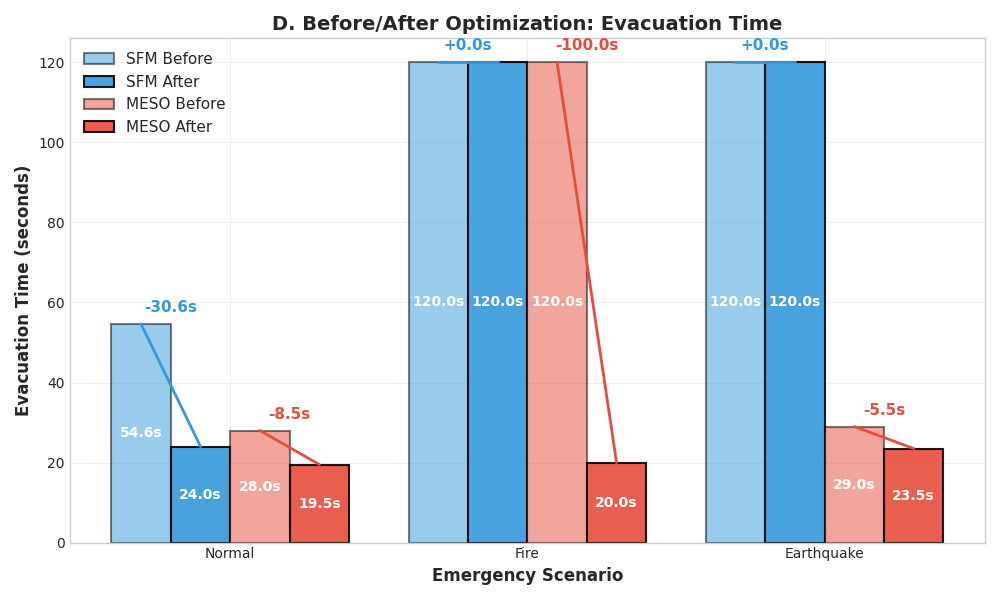
\includegraphics[width=0.48\textwidth]{before_after_optimization_evacuations_time.png}
\caption{Before/After Optimization: Evacuation Time}
\label{fig:evac_time_before_after}
\end{figure}

\begin{figure}[htbp]
\centering
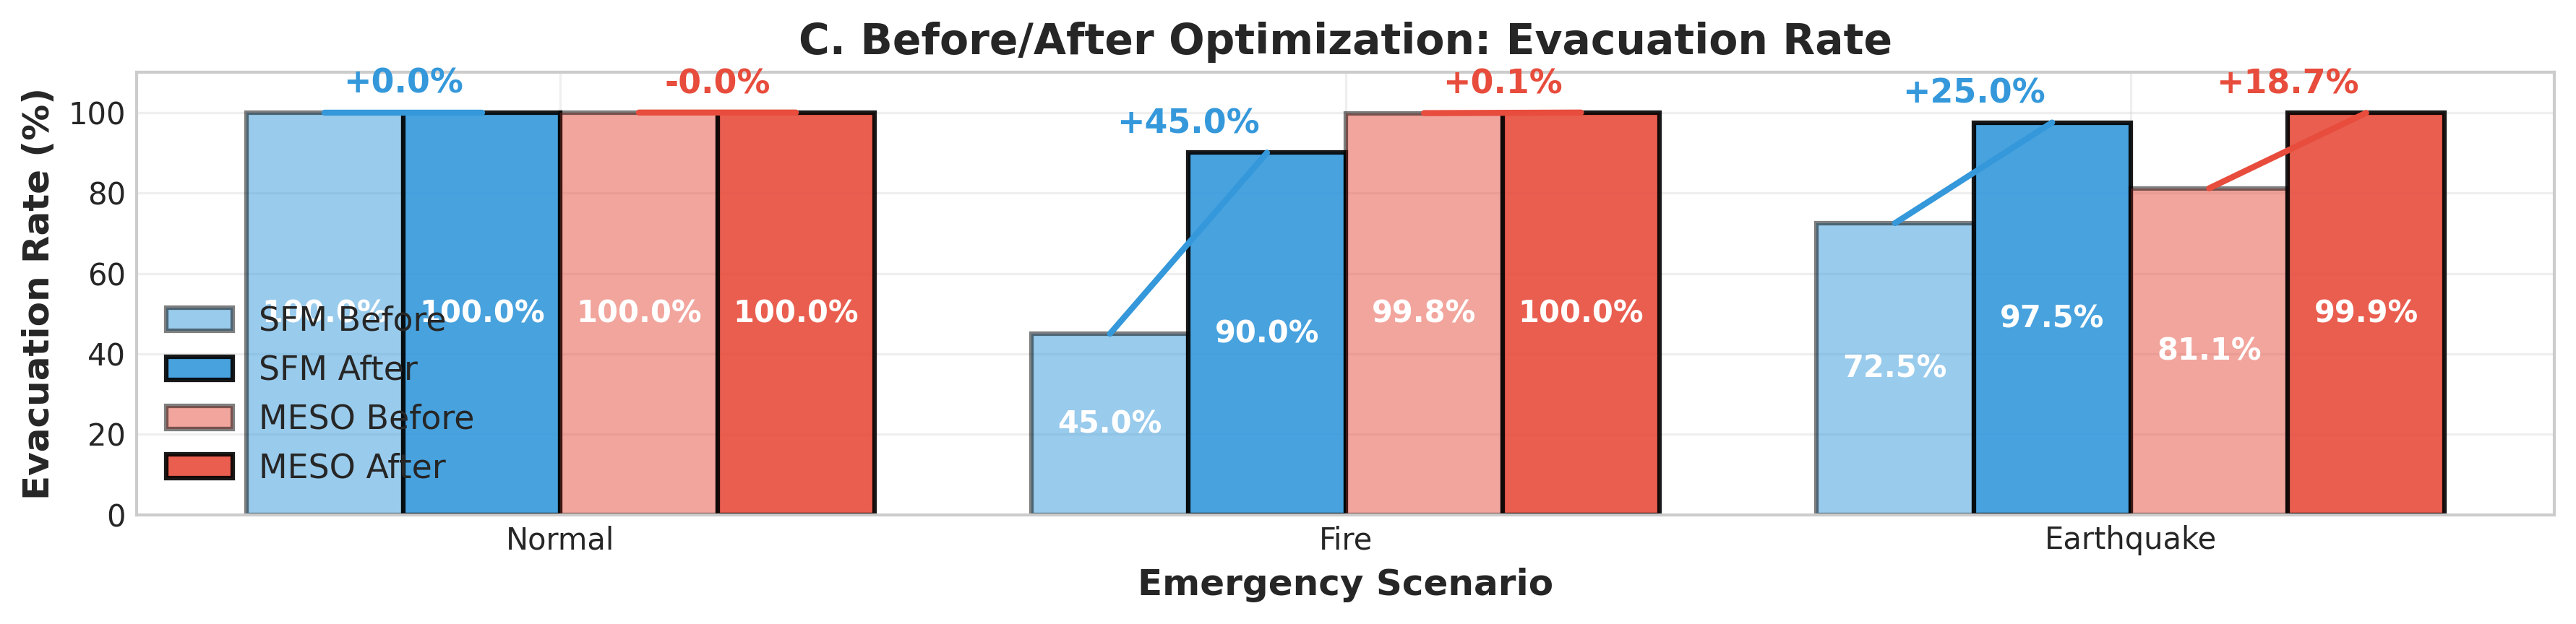
\includegraphics[width=0.48\textwidth]{before_after_optimization_evacuations_rate.png}
\caption{Before/After Optimization: Evacuation Rate}
\label{fig:evac_rate_before_after}
\end{figure}

\begin{figure}[htbp]
\centering
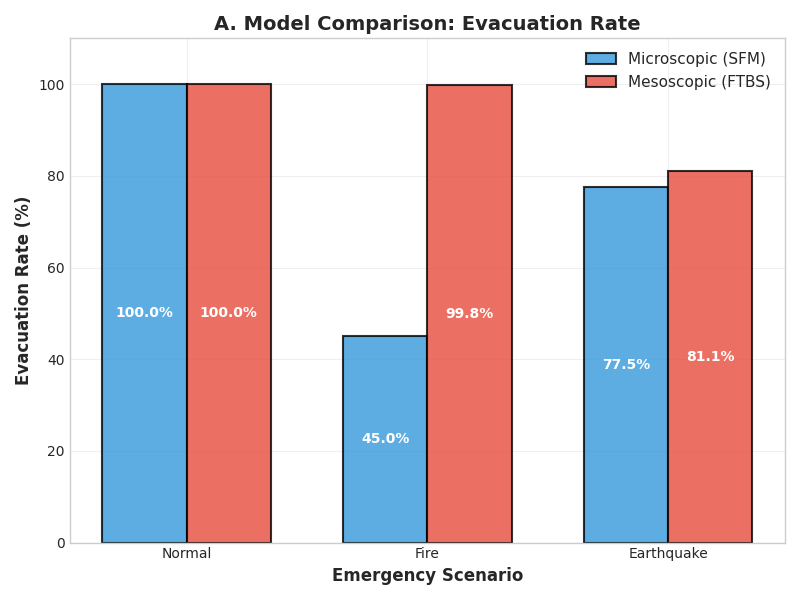
\includegraphics[width=0.4\textwidth]{model_comparison_evacuations_rate.png}
\caption{Model Comparison: Evacuation Rate}
\label{fig:rate_model_comparison}
\end{figure}

\begin{figure}[htbp]
\centering
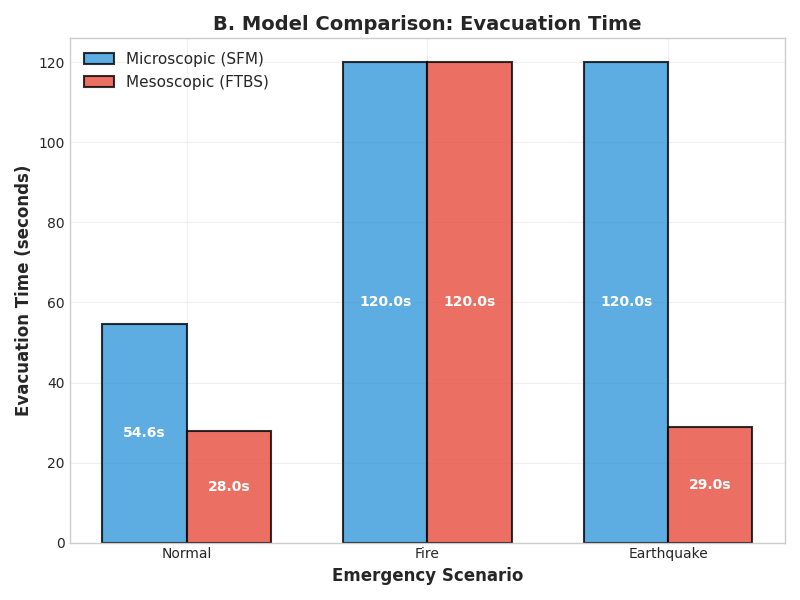
\includegraphics[width=0.4\textwidth]{model_comparison_evacuations_time.png}
\caption{Model Comparison: Evacuation Time}
\label{fig:time_model_comparison}
\end{figure}

\begin{figure}[htbp]
\centering
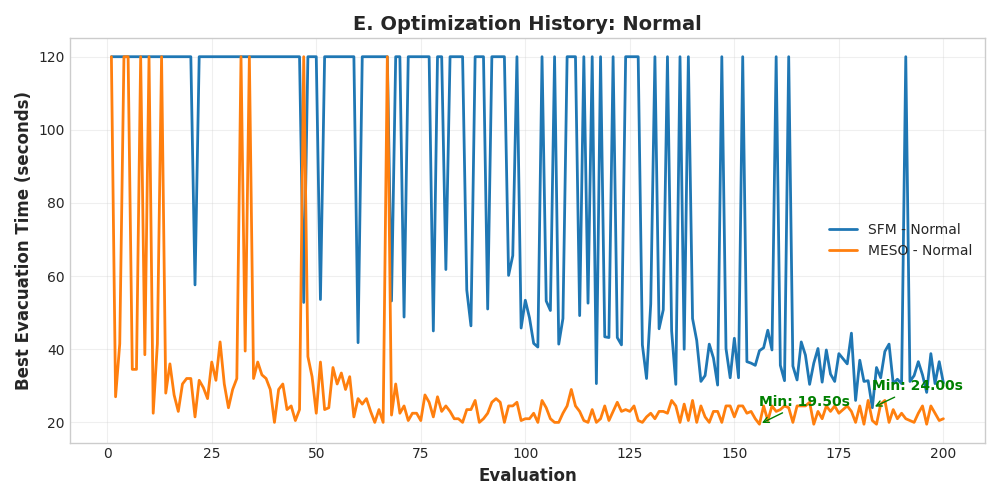
\includegraphics[width=0.48\textwidth]{optimization_history_normal.png}
\caption{Optimization History for Normal Scenario}
\label{fig:opt_history}
\end{figure}

\begin{figure}[htbp]
\centering
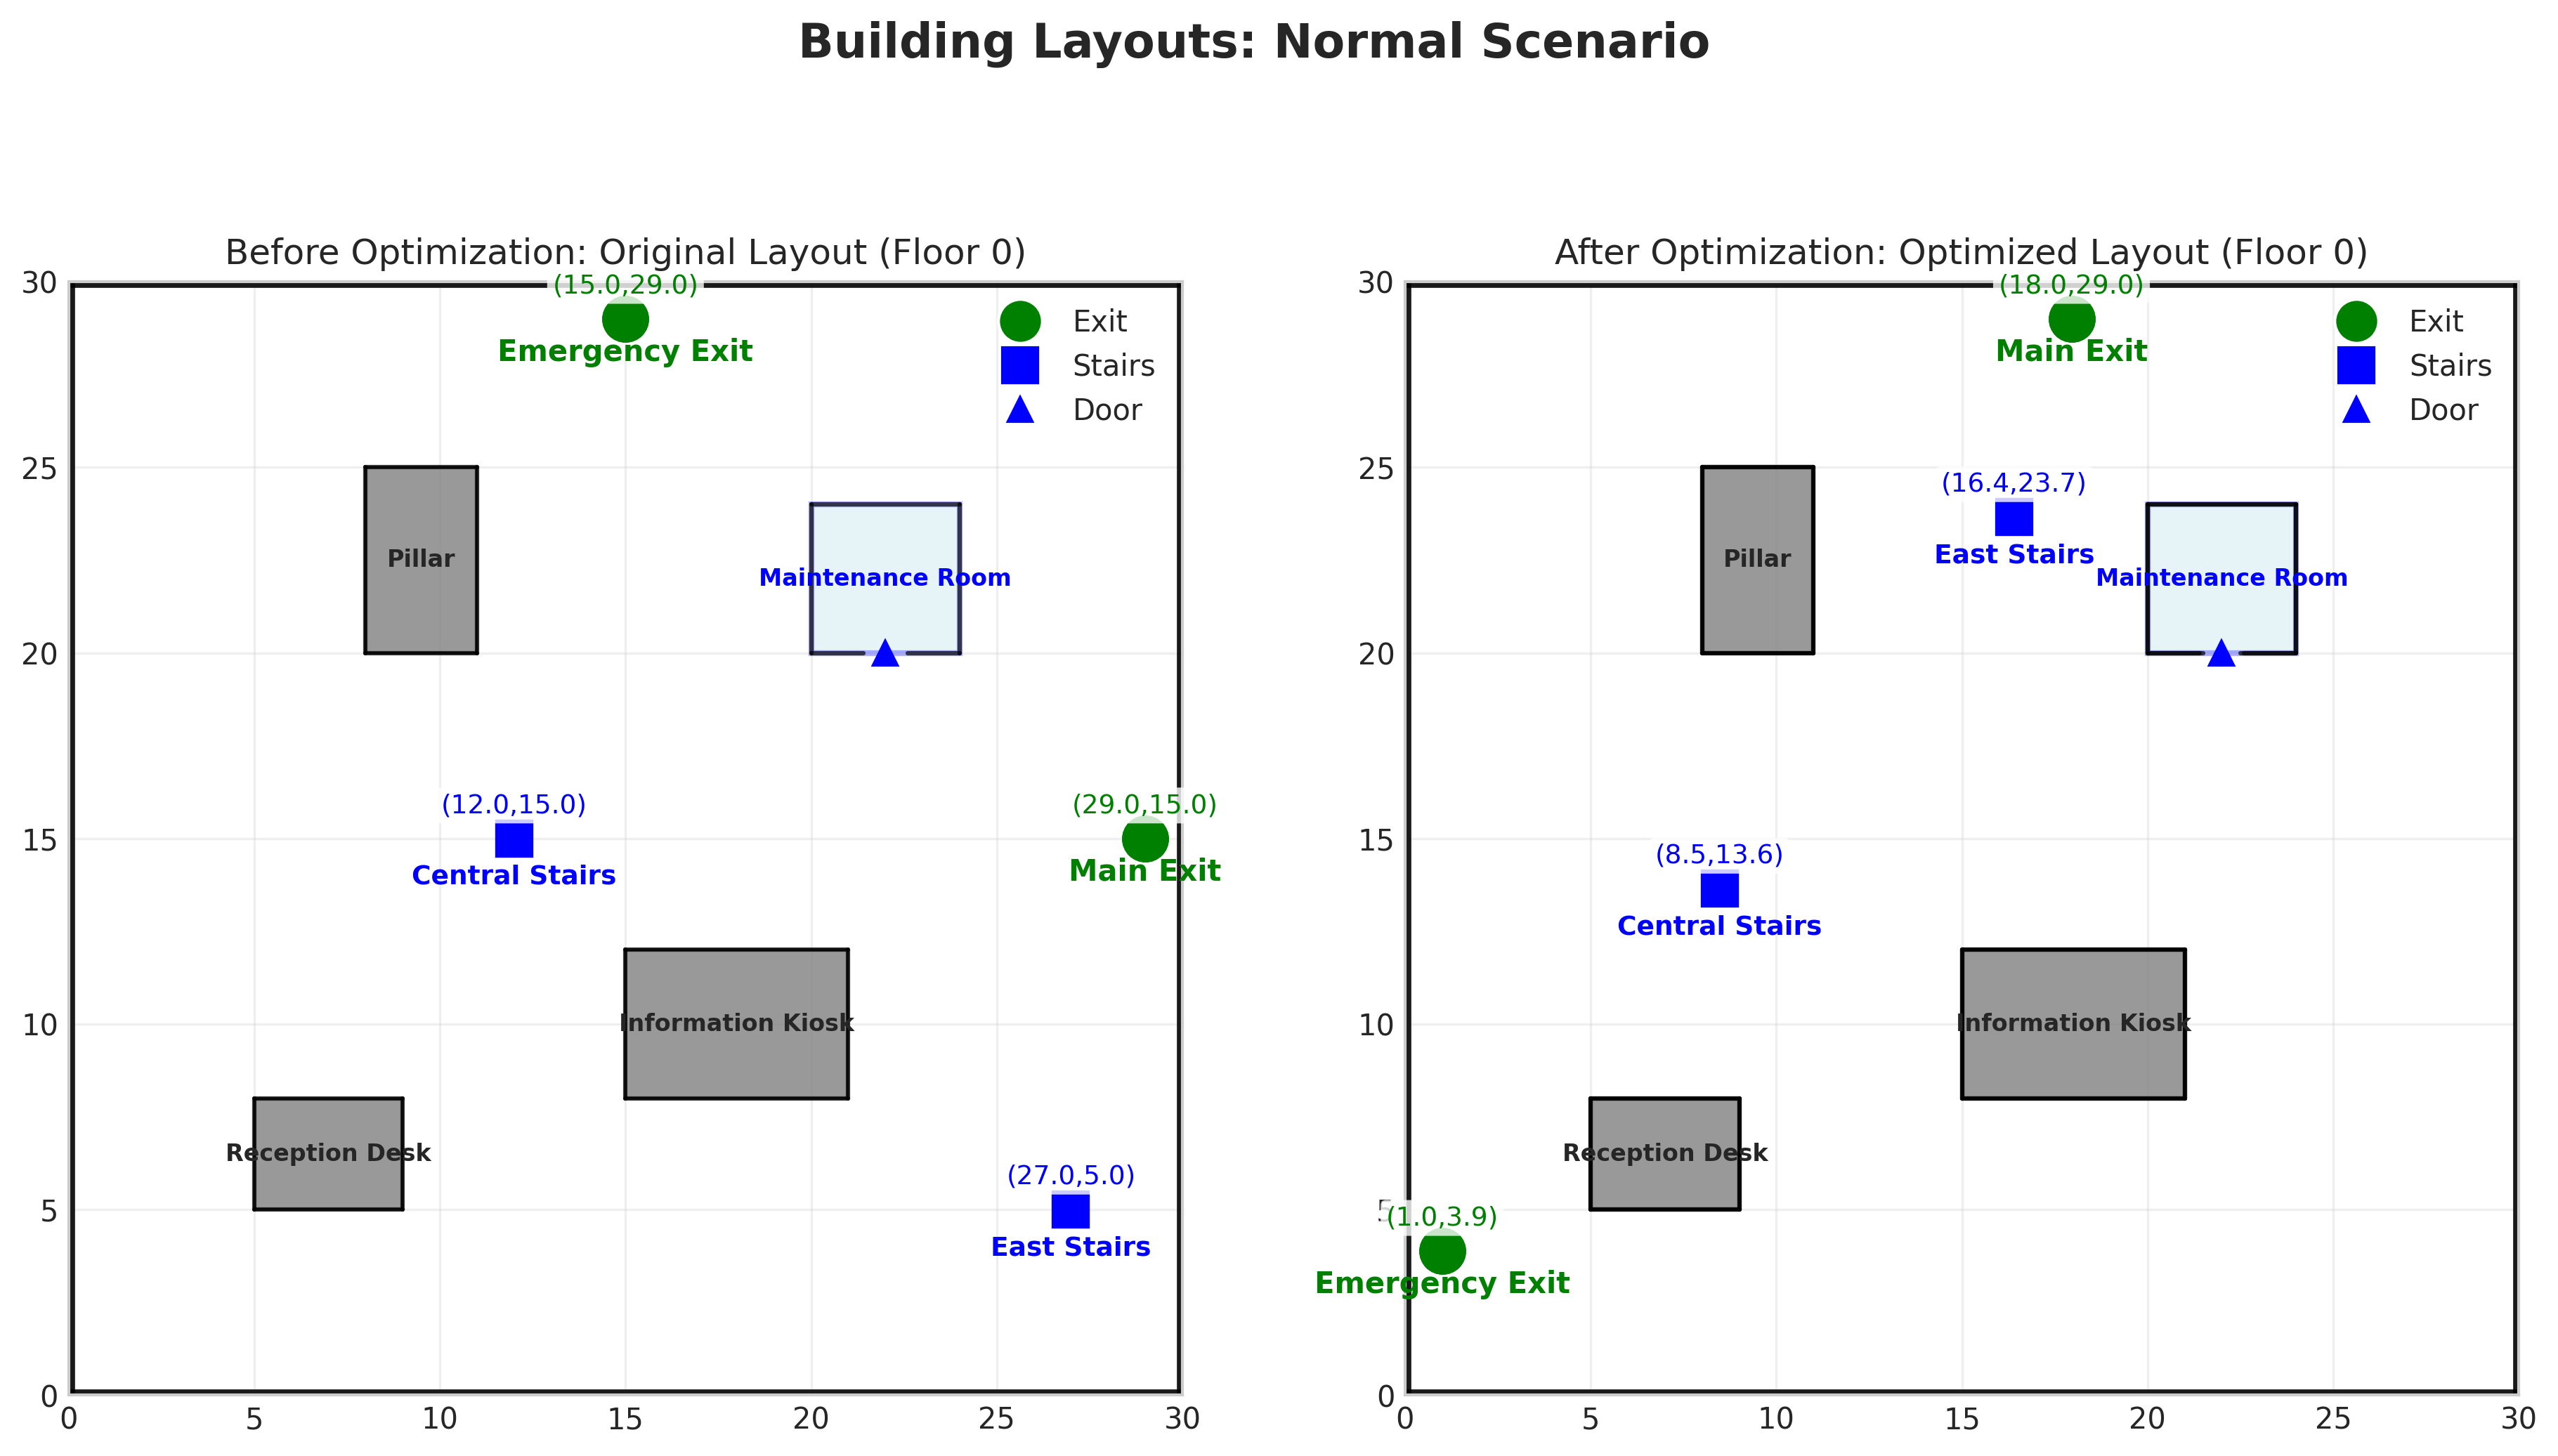
\includegraphics[width=0.48\textwidth]{building_layouts_normal_scenario.png}
\caption{Building Layouts: Normal Scenario}
\label{fig:layout_normal}
\end{figure}

\begin{figure}[htbp]
\centering
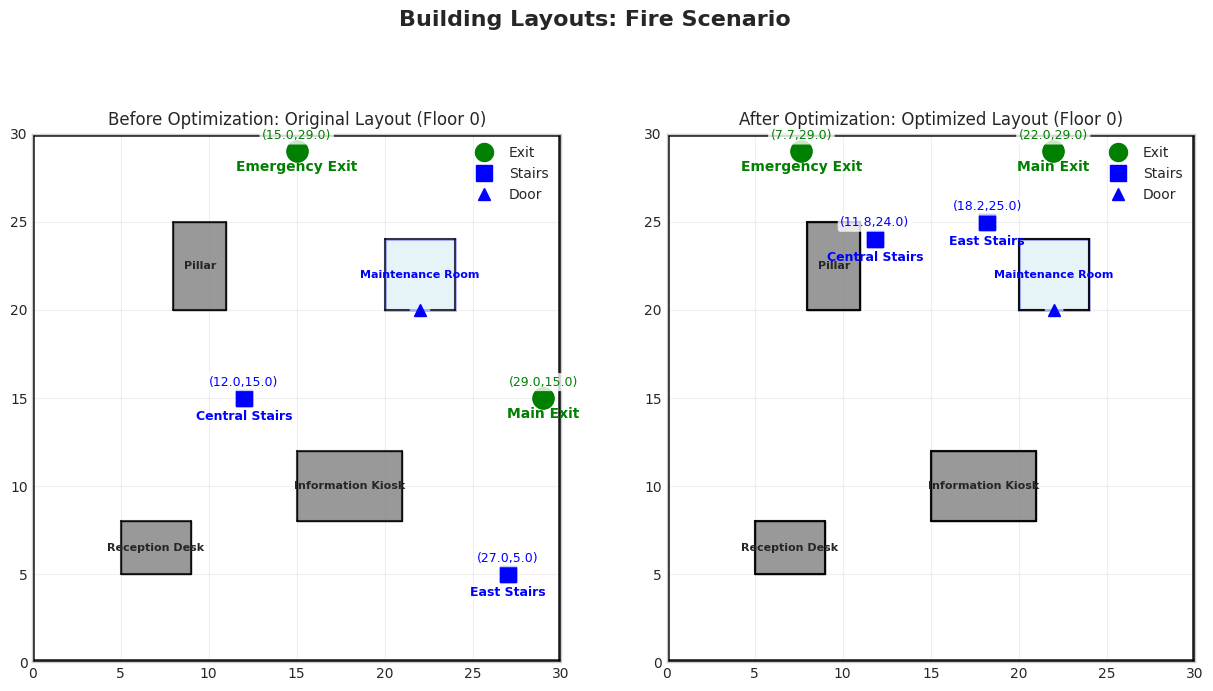
\includegraphics[width=0.48\textwidth]{building_layouts_fire_scenario.png}
\caption{Building Layouts: Fire Scenario}
\label{fig:layout_fire}
\end{figure}

\begin{figure}[htbp]
\centering
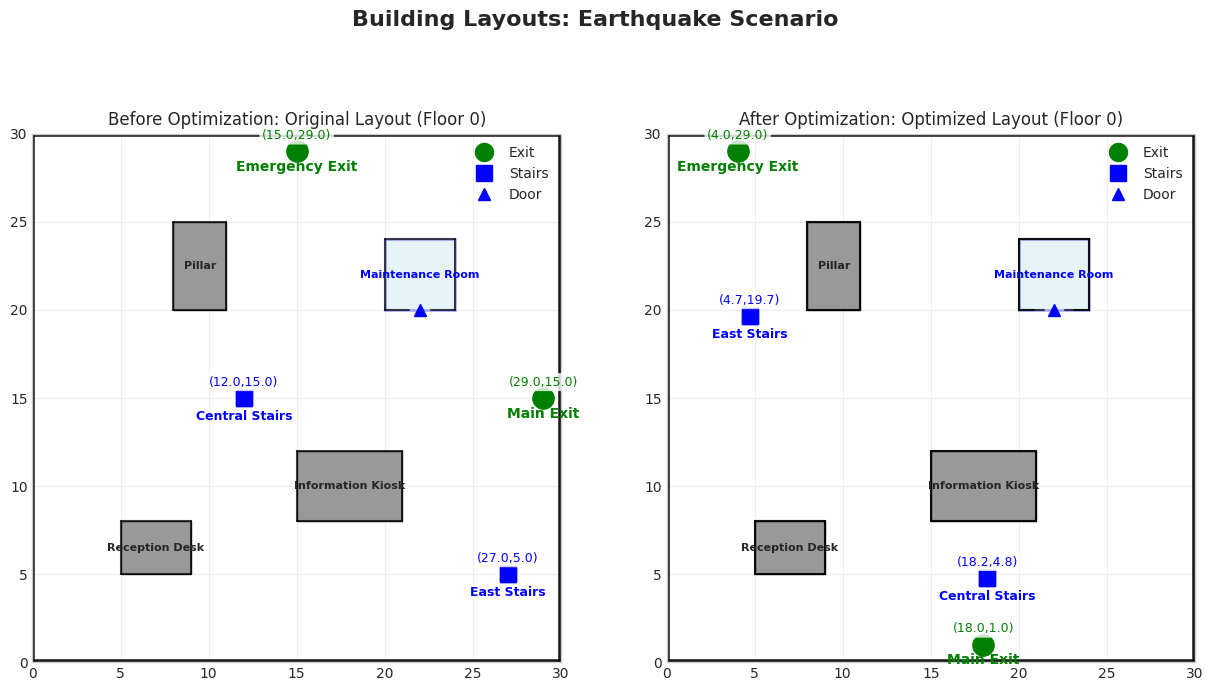
\includegraphics[width=0.48\textwidth]{building_layouts_earthquake_scenario.png}
\caption{Building Layouts: Earthquake Scenario}
\label{fig:layout_earthquake}
\end{figure}

\section{Conclusion}

This study presents a hybrid simulation-optimization framework for multi-floor building evacuation under normal and emergency scenarios. By integrating a microscopic Social Force Model and a mesoscopic FTBS model, we were able to simulate both detailed pedestrian behavior and rapid macroscopic flows.

Optimization using NSGA-II led to significant improvements, especially for the FTBS model under fire and earthquake scenarios. The optimized layouts reduced evacuation time by up to 30 seconds and improved evacuation rate by nearly 19\% in some cases.

The FTBS model demonstrated robustness in large-scale hazard scenarios, while SFM provided detailed local behavior insights. Future work will focus on real-world data validation, dynamic hazard evolution, and integration with IoT-enabled sensor feedback systems for real-time adaptive evacuation planning.


\begin{thebibliography}{99}

\bibitem{Deb2002} K. Deb, A. Pratap, S. Agarwal, and T. Meyarivan, “A fast and elitist multiobjective genetic algorithm: NSGA-II,” \emph{IEEE Transactions on Evolutionary Computation}, vol.~6, no.~2, pp.~182--197, 2002.
% Added for optimization: Introduces the NSGA-II algorithm, which is the core of optimization framework.

\bibitem{Gwynne1999} S. M. V. Gwynne, E. R. Galea, P. J. Lawrence, M. Owen, and L. Filippidis, “A review of the methodologies used in the computer simulation of evacuation from the built environment,” \emph{Building and Environment}, vol.~34, no.~6, pp.~741--749, 1999.
% Retained: Relevant for fire and smoke effects in evacuation modeling.

\bibitem{helbing1995} D. Helbing and P. Molnár, “Social force model for pedestrian dynamics,” \emph{Physical Review E}, vol.~51, no.~5, pp.~4282--4286, 1995.
% Retained: Foundational reference for the Social Force Model in microscopic simulations.

\bibitem{helbing2000} D. Helbing, I. Farkas, and T. Vicsek, “Simulating dynamical features of escape panic,” \emph{Nature}, vol.~407, no.~6803, pp.~487--490, 2000.
% Retained: Key for modeling panic behavior in the microscopic model under emergency scenarios.

\bibitem{Hoogendoorn2003} S. P. Hoogendoorn and P. H. L. Bovy, “Simulation of pedestrian flows by optimal control and differential games,” \emph{Optimal Control Applications and Methods}, vol.~24, no.~3, pp.~153--172, 2003.
% Added for mesoscopic model: Describes a mesoscopic approach to pedestrian flow modeling, relevant to network flow model.

\bibitem{Kirchner2002} A. Kirchner and A. Schadschneider, “Simulation of evacuation processes using a bionics-inspired cellular automaton model for pedestrian dynamics,” \emph{Physica A}, vol.~312, pp.~260--276, 2002.
% Retained: Supports the queue-based cost heuristic in microscopic model.

\bibitem{Kuligowski2010} E. D. Kuligowski, R. D. Peacock, and B. L. Hoskins, “A review of building evacuation models,” \emph{National Institute of Standards and Technology}, Technical Note 1680, 2010.
% Added for general context: Provides a comprehensive review of evacuation modeling approaches, covering microscopic, mesoscopic, and macroscopic models.

\bibitem{Treuille2006} A. Treuille, S. Cooper, and Z. Popović, “Continuum crowds,” \emph{ACM Transactions on Graphics}, vol.~25, no.~3, pp.~1160--1168, 2006.
% Added for mesoscopic model: Introduces a continuum-based approach to crowd modeling, which supports mesoscopic network flow model.

\bibitem{Yang2024} H. Yang, B. Wu, and G. Xu, “Modeling and experimental study on walking human-structure interaction systems subjected to earthquake excitations,” \emph{Journal of Sound and Vibration}, vol.~576, art.~118292, 2024.
% Retained: Relevant for earthquake scenario modeling in the microscopic model.

\end{thebibliography}

\end{document}
